% Emacs settings: -*-mode: latex; TeX-master: "manual.tex"; -*-

\chapter{The \MCS\ kernel and meta-language}
\label{s:kernel}
\index{Kernel|textbf}

Instrument definitions are written in a special \MCS\ meta-language which
is translated automatically by the \MCS\ compiler into a C program 
which is in turn compiled to an executable that
performs the simulation. The meta-language is custom-designed for neutron
scattering and serves two main purposes: (i) to specify the interaction of a
single neutron with a single optical component, and (ii) to build a
simulation by constructing a complete instrument from individual
components.

For maximum flexibility and efficiency, the meta-language is based on C.
Instrument geometry, propagation of neutrons between the different
components, parameters, data input/output etc.\ is handled in the
meta-language and by the \MCS\ compiler. Complex calculations are written in
C embedded in the meta-language description of the components. It is
possible to set up an instrument from existing components and
run a simulation without writing a single line of C code, working
entirely in the meta-language. On the other hand, the full power of the C
language is available for special-purpose setups in advanced
simulations, and for computing neutron trajectories in the components.

Apart from the meta-language, \MCS\ also includes a number of C library
functions and definitions that are useful for neutron ray-tracing
simulations. The definitions available for users coding components are
listed in appendix~\ref{c:kernelcalls}. The list includes functions for
computing the intersection between a flight-path and various objects
(such as cylinders and spheres), functions for generating random numbers
with various distributions, functions for reading or writing
informations from/to data files, convenient conversion
factors between relevant units, etc. \index{Library!Run-time}
\index{Library!Components!share}

The \MCS\ meta-language was designed to be readable, with a verbose
syntax and explicit mentioning of otherwise implicit information. The
recommended way to get started with the meta-language is to start by
looking at the examples supplied with \MCS, modifying them as necessary
for the application at hand.

\section{Notational conventions}

Simulations generated by \MCS\ use a semi-classical description of the
neutron to compute the neutron trajectory through the instrument and its
interaction with the different components. The effect of gravity is
taken  into account either in particular components, or more generaly
when setting an execution flag (\verb+-g+) to perform gravitation
computation. \index{Gravitation}

An instrument consists of a list of components through which the neutron
passes one after the other. The order of components is thus significant
since \MCS\ does not automatically check which component is the next to
interact with the neutron at a given point in the simulation.

The instrument is given a global, absolute coordinate system. In
addition, every component in the instrument has its own local coordinate
system that can be given any desired position and orientation (though
the position and orientation must remain fixed for the duration of a
single simulation). \index{Coordinate system}
By convention, the $z$ axis points in the direction of the beam, the $x$ axis
is perpendicular to the beam in the horizontal plane pointing left as seen
from the source, and the $y$ axis points upwards (see figure~\ref{f:axis}).
Nothing in \MCS\ enforces this convention, but if every component used
different conventions the user would be faced with a severe headache! It is
therefore recommended that this convention is followed by users implementing
new components.
\begin{figure}
  \begin{center}
    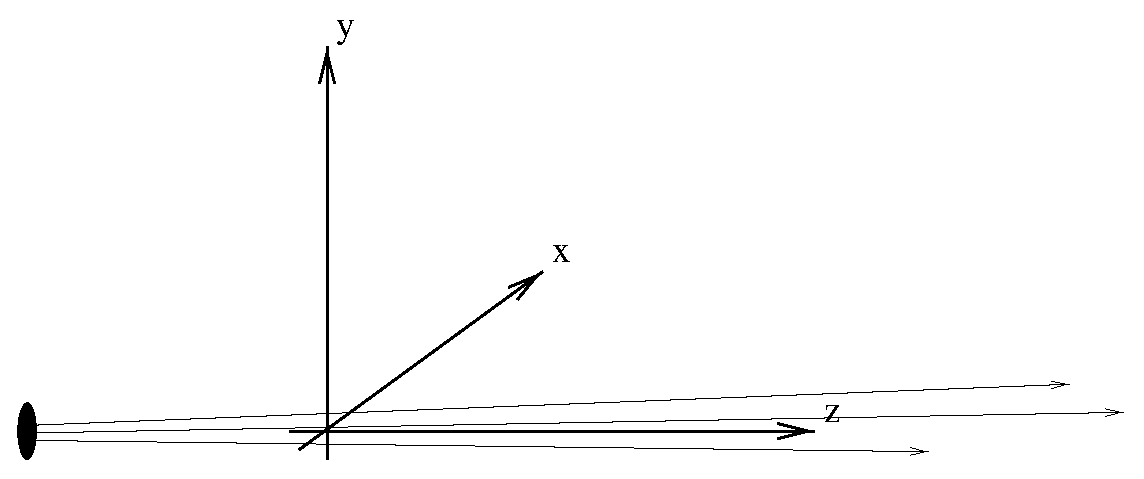
\includegraphics[width=0.8\textwidth]{figures/axis-conventions.eps}
  \end{center}
\caption{conventions for the orientations of the axis in simulations.}
\label{f:axis}
\end{figure}

\index{Neutron state and units}
In the instrument definitions, units of length (\textit{e.g}.\ component
positions) are given in meters and units of angles (\textit{e.g}.\ 
rotations) are given in degrees.  The state of the neutron is given by
its position $(x,y,z)$ in meters, its velocity $(v_x, v_y, v_z)$ in
meters per second, the time $t$ in seconds, and the two parameters
  %\footnote{The
  %spin is ignored in the current version 1.4 of \MCS. However, while not
  %documented in this manual, preliminary support for components that
  %handle the neutron spin is implemented using the POLARISATION
  %PARAMETER construct. We are currently working together with Trefor
  %Roberts at the ILL to get a correct handling of the spin.} 
$s_1$ and $s_2$ that are obsolete and should not be used. A three-component
representation of the spin, $\left( s_x, s_y, s_z \right)$, normalized to
one, is used. In addition, the outgoing neutron has an associated weight $p$
which is used to model fractional neutrons in the Monte Carlo simulation.
$p=0.2$ means that a single neutron following this path has a 20\% chance of
reaching the present position without being absorbed or scattered away from
the instrument. Alternatively, one may regard a ray of neutrons and $p$ is
the fraction of neutrons following the considered path.

\section{Syntaxical conventions}
\label{s:syntax}

Comments follow the normal C syntax ``\verb+/* ... */+''. C++ style
comments ``\verb+// ...+'' may also be used.
\index{Comments}

%For backward-compatibility
%with early versions, comments may also be written as a percentage sign
%followed by a space (``\verb*+% ...+''), but this is not recommended and
%will be removed in a future version.

Keywords are not case-sensitive, for example ``\verb+DEFINE+'',
``\verb+define+'', and ``\verb+dEfInE+'' are all equivalent. However, by
convention we always write keywords in uppercase to distinguish them
from identifiers and C language keywords. In contrast, \MCS\ 
identifiers (names), like C identifiers and keywords, \emph{are} case
sensitive, another good reason to use a consistent case convention for
keywords. All \MCS\ keywords are reserved, and thus should not be used 
as C variable names. The list of these reserved keywords is shown in table~\ref{t:keywords}. \index{Keyword|textbf}

\begin{table}
  \begin{center} 
    {\let\my=\\
    \begin{tabular}{|l|c|p{0.7\textwidth}|}
      \hline
      \texttt{Keyword} & Scope & Meaning \\
      \hline
      \texttt{ABSOLUTE} & I & Indicates that the AT and ROTATED keywords are in the absolute coordinate system. \\
      \texttt{AT} & I & Indicates the position of a component in an instrument definition. \\
      \texttt{DECLARE} & I,C & Declares C internal instrument or component variables. \\
      \texttt{DEFINE} & I,C & Starts an instrument or component definition. \\
      \texttt{- INSTRUMENT} & & \\
      \texttt{- COMPONENT} & & \\
      \texttt{DEFINITION} & C & Defines component parameters that are constants (like C \#define). \\
      \texttt{END} & I,C & Ends the instrument or component definition. \\
      \texttt{EXTEND} & I & Extends the TRACE section of a component in an instrument definition. \\
      \texttt{FINALLY} & I,C & Embeds C code to execute when simulation ends (also executes the SAVE section). \\
      \texttt{GROUP} & I & Defines an exclusive group of components. \\
      \texttt{\%include} & I,C & Imports an instrument part, a component or a piece of C code (when within embedded C). \\
      \texttt{INITIALIZE} & I,C & Embeds C code to be executed when starting. \\
      \texttt{MCDISPLAY} & C & Embeds C code to display a geometric  representation of a component. \\
      \texttt{OUTPUT} & C & Defines internal variables to be public and protected symbols (usually all those of DECLARE).\\
      \texttt{PARAMETERS} & C & Defines a class of component parameter. \\
      \texttt{POLARISATION} & C & Defines neutron polarisation coordinates. \\
      \texttt{PREVIOUS} & C & Refers to a previous component position/orientation. \\
      \texttt{RELATIVE} & I & Indicates that the AT and ROTATED keywords are relative to an other component. \\
      \texttt{ROTATED} & I & Indicates the orientation of a component in an instrument definition. \\
      \texttt{SAVE} & I,C & Embedded C code to execute when saving data. \\
      \texttt{SETTING} & C & Defines component parameters that are
      variables (double, int, char*). \\
      \texttt{SHARE} & C & Declares global functions and variables to be used by all components. \\
      \texttt{STATE} & C & Defines neutron state coordinates. \\
      \texttt{TRACE} & I,C & Lists the components or embedded C code to execute during simulation. \\
      \hline
    \end{tabular}
    \caption{Reserved \MCS\ keywords. 
    Scope is 'I' for instrument and 'C' for component definitions.}
    \label{t:keywords}
    }
  \end{center}
\end{table}

It is possible, and usual, to split the input instrument definition
across several different files. For example, if a component is not
explicitly defined in the instrument,
\MCS\ will search for a file containing the component definition in the
standard component library (as well as in the current directory and any
user-specified search directories, see section~\ref{s:files}). It is
also possible to explicitly include another file using a line of the
form \index{Keyword!\%include}
\begin{verbatim}
    %include "file"
\end{verbatim}
Beware of possible confusion with the C language ``\verb+#include+''
statement, especially when it is used in C code embedded within the
\MCS\ meta-language. Files referenced with ``\verb+%include+'' are read
when the instrument is translated into C by the \MCS\ compiler, and must
contain valid \MCS\ meta-language input (and possibly C code). Files referenced with
``\verb+#include+'' are read when the C compiler generates an
executable from the generated C code, and must contain valid C.

Embedded C code is used in several instances in the \MCS\
meta-language. Such code is copied by the \MCS\ compiler into the
generated simulation C program. Embedded C code is written by putting it
between the special symbols \verb|%{| and \verb|%}|, as follows:
\begin{quote}
  \verb|%{| \\
  \hbox to 3em{}\ldots Embedded C code \ldots \\
  \verb|%}|
\end{quote} \index{Embedded C code}
The ``\verb|%{|'' and ``\verb|%}|'' must appear on a line by themselves (do not add comments after).
Additionally, if a ``\verb+%include+'' statement is found \emph{within} an embedded C code block, the specified file will be included from the 'share' directory of the standard component library \index{Library!Components!share} (or from the
current directory and any user-specified search directories) as a C library, just like the usual ``\verb+#include+'' \emph{but only once}. For instance, if many components require to read data from a file, they may all ask for ``\verb+%include "read_table-lib"+'' \index{Library!read\_table-lib (Read\_Table)} without duplicating the code of this library. If the file has no extension, both \verb+.h+ and \verb+.c+ files will be searched and included, otherwise, only the specified file will be imported. The \MCS\ 'run-time' shared 
library is included by default (equivalent to ``\verb+%include "mcstas-r"+'' in the \texttt{DECLARE} section). \index{Library!Run-time}
For an
example of \texttt{\%include}, see the monitors/Monitor\_nD component.


\section{Writing instrument definitions}
\label{s:instrdefs}
\index{Instruments}

The purpose of the instrument definition is to specify a sequence of
components, along with their position and parameters, which together
make up an instrument. Each component is given its own local coordinate
system, the position and orientation of which may be specified by its
translation and rotation relative to another component. An example is
given in section~\ref{s:vanadium_example.instr} and some additional
examples of instrument definitions can be found on the McStas
web-page~\cite{mcstas_webpage} and in the \texttt{example} directory.

%An instrument definition looks as follows:


\subsection{The instrument definition head}

\begin{quote}
  \texttt{DEFINE} \texttt{INSTRUMENT} \textit{name} $(a_1, a_2, \ldots)$
\end{quote} \index{Keyword!DEFINE!INSTRUMENT}
This marks the beginning of the definition. It also gives the name of
the instrument and the list of instrument parameters. Instrument
parameters describe the configuration of the instrument, and usually
correspond to setting parameters of the components. A motor position is
a typical example of an instrument parameter. The input parameters of
the instrument constitute the input that the user (or possibly a
front-end program) must supply when the
generated simulation is started. 

\index{Parameters!Instruments}
By default, the parameters will be floating point numbers, and will have
the C type \verb+double+ (double precision floating point). The type of
each parameter may optionally be declared to be \verb+int+ for the C
integer type or \verb+char *+ for the C string type. The name
\verb+string+ may be used as a synonym for \verb+char *+, and floating
point parameters may be explicitly declared using the name
\verb+double+. The following example illustrates all possibilities:
\begin{quote}
  \texttt{DEFINE INSTRUMENT test(d1, double d2, int i, char *s1, string s2)}
\end{quote}
Here \verb+d1+ and \verb+d2+ will be floating point parameters of C type
\verb+double+, \verb+i+ will be an integer parameter of C type
\verb+int+, and \verb+s1+ and \verb+s2+ will be string parameters of C
type \verb+char *+. 
\index{Parameters!Optional, default value}
The parameters of an instrument may be given default values. Parameters with default values are called \emph{optional
  parameters}, and need not be given an explicit value when the
instrument simulation is executed. When executed without any parameter value in the command line (see section~\ref{s:run-sim}), the instrument asks for all parameter values, but pressing the \verb+Return+ key selects the default value (if any). When used with parameter values in the command line, all non specified parameters will have their value set to the default one (if any). A parameter is given a
default value using the syntax ``\textit{param}\texttt{ = }\textit{value}''.
For example
\begin{quote}
  \texttt{DEFINE INSTRUMENT test(d1 = 1, string s2="hello")}
\end{quote}
Here \verb+d1+ is an optional parameter and if no value is given
explicitly, ``1'' will be used.

Optional parameters can greatly increase the convenience for users of
instruments for which some parameters are seldom changed or of unclear signification to the user. Also, if all instrument parameters have default values, then the simple command \verb+mcdisplay+ \verb+test.instr+ will show the instrument view without requesting any other input, which is usually a good starting point to study the instrument design.

\subsection{The \texttt{DECLARE} section}
\index{Keyword!DECLARE}
\label{s:declare}

\begin{quote}
  \texttt{DECLARE} \\
  \verb|%{| \\
  \hbox to 3em{}\ldots C declarations of global variables etc. \ldots \\
  \verb|%}|
\end{quote} \index{Embedded C code}
This gives C declarations that may be referred to in the rest of the
instrument definition. A typical use is to declare global variables or
small functions that are used elsewhere in the instrument. The \verb+%include ''file''+ keyword may be used to import a specific
component definition or a part of an instrument. The \texttt{DECLARE} section is optional.

\subsection{The \texttt{INITIALIZE} section}
\index{Keyword!INITIALIZE}
\label{s:initialize}

\begin{quote}
  \texttt{INITIALIZE} \\
  \verb|%{| \\
  \hbox to 3em{}\ldots C initializations. \ldots \\
  \verb|%}|
\end{quote} \index{Embedded C code}
This gives code that is executed when the simulation starts. This section is
optional.


\subsection{The \texttt{TRACE} section}
\index{Keyword!TRACE}
\label{s:trace}

The \texttt{TRACE} keyword starts a section giving the list of
components that constitute the instrument.
Components are declared like this:
\begin{quote}
  \texttt{COMPONENT} $\textit{name} =
    \textit{comp}(p_1 = e_1, p_2 = e_2, \ldots)$
\end{quote}
\index{Components}
\index{Keyword!COMPONENT} \index{Parameters!Setting}
\index{Parameters!Definition}
This declares a component named \textit{name} that is an instance of the
component definition named \textit{comp}. The parameter list gives the
setting and definition parameters for the component. The expressions $e_1,
e_2, \ldots$ define the values of the parameters. For setting parameters
arbitrary ANSI-C expressions may be used, while for definition parameters
only \emph{constant} numbers, strings, names of instrument parameters, or names
of C identifiers are allowed (see section~\ref{s:comp-header} for details of
the difference between definition and setting parameters). To assign the
value of a general expression to a definition parameter, it is necessary to
declare a variable in the \texttt{DECLARE} section, assign the value to the
variable in the \texttt{INITIALIZE} section, and use the variable as the
value for the parameter.

The \MCS\ program takes care to rename parameters appropriately in the
output so that no conflicts occur between different component
definitions or between component and instrument definitions. It is thus
possible (and usual) to use a component definition multiple times
in an instrument description.

The \MCS\ compiler will automatically search for a file containing a
definition of the component if it has not been declared previously. The
definition is searched for in a file called ``{\it name\/}{\tt .comp}'',
``{\it name\/}{\tt .cmp}'', or ``{\it name\/}{\tt .com}''. See
section~\ref{s:files} for details on which directories are searched. This
facility is often used to refer to existing component definitions in
standard component libraries. It is also possible to write component
definitions in the main file before the instrument definitions, or to
explicitly read definitions from other files using \verb+%include+ 
(not within embedded C blocks).

The position of a component is specified using an \texttt{AT} modifier
following the component declaration:
\index{Keyword!AT} \index{Keyword!RELATIVE} \index{Keyword!ABSOLUTE}
\begin{quote}
  \texttt{AT} $(x,y,z)$ \texttt{RELATIVE} \textit{name}
\end{quote}
This places the component at position $(x,y,z)$ in the coordinate system
of the previously declared component \textit{name}. Placement may also
be absolute (not relative to any component) by writing
\begin{quote}
  \texttt{AT} $(x,y,z)$ \texttt{ABSOLUTE}
\end{quote}
Any C expression may be used for $x$, $y$, and $z$. The \texttt{AT}
modifier is required.
Rotation is achieved similarly by writing \index{Keyword!ROTATED}
\begin{quote}
  \texttt{ROTATED} $(\phi_x,\phi_y,\phi_z)$ \texttt{RELATIVE} \textit{name}
\end{quote}
This will result in a coordinate system that is rotated first the angle
$\phi_x$ (in degrees) around the $x$ axis, then $\phi_y$ around the $y$ axis, and finally
$\phi_z$ around the $z$ axis. Rotation may also be specified using
\texttt{ABSOLUTE} rather than \texttt{RELATIVE}. If no rotation is
specified, the default is $(0,0,0)$ using the same relative or absolute
specification used in the \texttt{AT} modifier.

The \texttt{PREVIOUS} \index{Keyword!PREVIOUS} keyword is a generic name to refer to the previous component in the simulation. Moreover, the \texttt{PREVIOUS(n)} keyword will refer to the $n$-th previous component, starting from the current component, so that \texttt{PREVIOUS} is equivalent to \texttt{PREVIOUS(1)}. This keyword should be used after the \texttt{RELATIVE} keyword, but not for the first component instance of the instrument description. Invalid \texttt{PREVIOUS} references will be assumed to be absolute placement. 

The order and position of components in the \texttt{TRACE} section does not
allow components to overlap, except for particular cases.
Indeed, many components of the \MCS\ library \index{Library!Components} start
by propagating the neutron event to the begining of the component itself.
Anyway, when the corresponding propagation time is found to be negative
({\it i.e.} the neutron is already \emph{after} the component, and has thus
passed the 'active' position), the neutron event is ABSORBed, resulting in a zero intensity and event counts after a given position. Such situations
may arise e.g. when positioning some components not one after the other (nested, in parallel, or overlapping), for
instance in a multiple crystal monochromator (they are then side by side). One
would then like the neutron to interact with \emph{one of} the components and
then continue after this group of components. In order to handle such
arrangements, groups are defined by appending the \texttt{GROUP} modifier
\begin{quote}
  \texttt{GROUP} \textit{name}
\end{quote}
to all involved component declarations. \index{Keyword!GROUP}
All components of the same named group are tested one after the other, until one of them interacts (uses the SCATTER macro \index{Library!Run-time!SCATTER}). The selected component acts on the neutron, and the rest of the group is skipped. Such groups are thus exclusive (only one of the elements is active).
If no component of the group could intercept the neutron, it is ABSORBed. If you wish not to absorb these neutrons, you may end each group by a large monitor, which will eventually catch neutrons that were not caught by previous components of the group.

It is sometimes desirable to slighlty modify an existing component of the \MCS\ library. One would usually make a copy of the component, and extend the code of its \texttt{TRACE} section. \MCS\ provides an easy way to change the behaviour of existing components in an instrument definition without duplicating files, using the \texttt{EXTEND} modifier \index{Keyword!EXTEND}
\begin{quote}
  \texttt{EXTEND} \\
  \verb|%{| \\
  \hbox to 3em{}\ldots C code executed after the component TRACE section \ldots \\
  \verb|%}|
\end{quote} \index{Embedded C code}
The embeded C code is appended to the component \texttt{TRACE} section, and all its internal variables may be used.
This component declaration modifier is of course optional. Within a \texttt{GROUP}, \emph{all} \texttt{EXTEND} sections of the group are executed. In order to discriminate components that are active from those that are skipped, one may use the SCATTERED flag, which is set to zero when entering each component or group, and incremented when the neutron is SCATTERed, as in the following example \index{Library!Run-time!SCATTER} \index{Library!Run-time!SCATTERED}
\begin{quote}
  \texttt{COMPONENT} $\textit{name0} =
    \textit{comp}(p_1 = e_1, p_2 = e_2, \ldots)$ \\
  \hbox to 1em{} \texttt{AT} $(0,0,0)$ \texttt{ABSOLUTE} \\
  \texttt{COMPONENT} $\textit{name1} =
    \textit{comp}(\ldots)$ \\
  \hbox to 1em{} \texttt{AT} $(x,y,z)$ \texttt{RELATIVE} \textit{name0} \\
  \hbox to 1em{} \texttt{ROTATED} $(\phi_x,\phi_y,\phi_z)$ \texttt{RELATIVE} \textit{name0} \\
  \hbox to 1em{} \texttt{GROUP} \textit{GroupName} \texttt{EXTEND} \\
  \hbox to 1em{} \verb|%{| \\
  \hbox to 3em{} \verb+if (SCATTERED) printf("I scatter"); else printf("I do not scatter");+\\
  \hbox to 1em{} \verb|%}| \\
  \texttt{COMPONENT} $\textit{name2} =
    \textit{comp}(\ldots)$ \\
  \hbox to 1em{} \texttt{AT} $(x,y,z)$ \texttt{RELATIVE} \textit{name0} \\
  \hbox to 1em{} \texttt{ROTATED} $(\phi_x,\phi_y,\phi_z)$ \texttt{RELATIVE} \textit{name0} \\
  \hbox to 1em{} \texttt{GROUP} \textit{GroupName}
\end{quote}
Components \emph{name1} and \emph{name2} are at the same position. If the first one intercepts the neutron (and has a SCATTER within its \texttt{TRACE} section), the SCATTERED variable becomes true, the code extension will result in printing "I scatter", and the second component will be skipped.
Thus, we recommand to make use of the SCATTER keyword each time a component 'uses' the neutron (scatters, detects, \ldots).


\subsection{The \texttt{SAVE} section}
\index{Keyword!SAVE}
\label{s:save}

\begin{quote}
  \texttt{SAVE} \\
  \verb|%{| \\
  \hbox to 3em{}\ldots C code to execute each time a temporary save is required \ldots \\
  \verb|%}|
\end{quote} \index{Signal handler!USR2 signal}
This gives code that will be executed when the simulation is requested to save data, for instance when receiving a USR2 signal (on Unix systems), or using the \verb+Progress_bar+ component with intermediate savings. This section is optional.

\subsection{The \texttt{FINALLY} section}
\index{Keyword!FINALLY}
\label{s:finally}

\begin{quote}
  \texttt{FINALLY} \\
  \verb|%{| \\
  \hbox to 3em{}\ldots C code to execute at end of simulation \ldots \\
  \verb|%}|
\end{quote}
This gives code that will be executed when the simulation has
ended. When existing, the \texttt{SAVE} section is first executed. This section is optional.
A simulation may be requested to end before all neutrons have been traced when recieving a TERM or INT signal (on Unix systems), or with Control-C.
\index{Signal handler!TERM signal} \index{Signal handler!INT signal}


\subsection{The end of the instrument definition}
\label{s:end}
\index{Keyword!END}

The end of the instrument definition is marked using the keyword
\begin{quote}
  \texttt{END}
\end{quote}

\subsection{Code for the instrument \texttt{vanadium\_example.instr}}
\label{s:vanadium_example.instr}
An instrument definition taken from the \texttt{examples} directory is
given as an example.
\smallverbatimfile{../mcstas/lib/examples/vanadium_example.instr}

\section{Writing component definitions}
\label{s:compdefs}

The purpose of a component definition is to model the interaction of a
neutron with the component. Given the state of the incoming neutron, the
component definition calculates the state of the neutron when it leaves
the component.  The calculation of the effect of the component on the
neutron is performed by a block of embedded C code. 
One example of a component definition is given in section~\ref{s:slit}, and all
component definitions can be found on the McStas web-page~\cite{mcstas_webpage}.

There exists a large number of functions and constants available in
order to write efficient components. Look at the appendix~\ref{c:kernelcalls} for neutron propagation functions, geometric intersection time computations, vector operators, random number and vector generation, physical constants, coordinate retrieval and operations, file generation routines (for monitors), data file reading, \ldots

%A component definition looks as follows:


\subsection{The component definition header}
\label{s:comp-header}

\begin{quote}
  \texttt{DEFINE} \texttt{COMPONENT} \textit{name}
\end{quote}
\index{Keyword!DEFINE!COMPONENT}
This marks the beginning of the definition, and defines the name of the
component.
\begin{quote}
  \texttt{DEFINITION} \texttt{PARAMETERS} $(d_1, d_2, \ldots)$ \\
  \texttt{SETTING} \texttt{PARAMETERS} $(s_1, s_2, \ldots)$
\end{quote}
\index{Keyword!DEFINITION PARAMETERS}
\index{Keyword!SETTING PARAMETERS}
This declares the definition and setting parameters of the component.
The parameters define the characteristics of the component, and can be
accessed from the \verb+SAVE+, \verb+FINALLY+, and \verb+MCDISPLAY+ sections (see below), 
as well as in \verb+EXTEND+ sections of the instrument definition (see section~\ref{s:instrdefs}).
\index{Parameters!Setting}
\index{Parameters!Definition}

Setting parameters are translated into C variables usually of type
\verb+double+ in the generated simulation program, so they are usually
numbers. Definition parameters are translated into \verb+#define+ macro
definitions, and so can have any type, including strings, arrays, and
function pointers.

However, because of the use of \verb+#define+, definition parameters
suffer from the usual problems with C macro definitions. Also, it is not
possible to use a general C expression for the value of a definition
parameter in the instrument definition, only constants and variable
names may be used. For this reason, setting parameters should be used
whenever possible.

There are a few cases where the use of definition parameters instead of
setting parameters makes sense. If the parameter is not numeric, nor a character string ({\em i.e.} an
array, for example), a setting parameter cannot be
used. Also, because of the use of \verb+#define+, the C compiler can
treat definition parameters as constants when the simulation is
compiled. For example, if the array sizes of a multidetector are
definition parameters, the arrays can be statically allocated in the
component \verb+DECLARE+ section. If setting parameters were used, it
would be necessary to allocate the arrays dynamically using {\em e.g.}\ 
\verb+malloc()+.

Setting parameters may optionally be declared to be of type \verb+int+ and \verb+char *+, just as in the instrument definition (see section~\ref{s:instrdefs}).

\begin{quote}
  \texttt{OUTPUT} \texttt{PARAMETERS} $(s_1, s_2, \ldots)$
\end{quote}
\index{Keyword!OUTPUT PARAMETERS}
This declares a list of C identifiers that are output parameters for the
component. Output parameters are used to hold values that are computed
by the component itself, rather than being passed as input. This could
for example be a count of neutrons in a detector or a constant that is
precomputed to speed up computation. Output
parameters will typically be declared as C variables in the
\texttt{DECLARE} section, see section~\ref{s:comp-declare} below for an
example.

The \texttt{OUTPUT} \texttt{PARAMETERS} section is optional.

\begin{quote}
  \texttt{STATE} \texttt{PARAMETERS} $(x,y,z,v_x,v_y,v_z,t,s_1,s_2,p)$
\end{quote}
\index{Keyword!STATE PARAMETERS}
This declares the parameters that define the state of the incoming
neutron. The task of the component code is to assign new values to these
parameters based on the old values and the values of the definition and
setting parameters. Note that $s_1$ and $s_2$ are obsolete and cannot be used.

\begin{quote}
  \texttt{POLARISATION} \texttt{PARAMETERS} $(s_x,s_y,s_z)$
\end{quote}
\index{Keyword!POLARISATION PARAMETERS}
This line is necessary only if the component handles polarisation of neutrons
and thus modifies the spin vector. For an instrument to handle polarisation
correctly, it is only required that {\em one} of the components contains this
line.

\subsubsection{Optional component parameters}
\index{Parameters!Optional, default value}

Just as for instrument parameters, the definition and setting parameters of a
component may be given a default value. Parameters with default values are
called \emph{optional parameters}, and need not be given an explicit value when
the component is used in an instrument definition. A parameter is given a
default value using the syntax ``\textit{param}\texttt{ = }\textit{value}''.
For example
\begin{quote}
  \texttt{SETTING PARAMETERS (radius, height, pack = 1)}
\end{quote}
Here \verb+pack+ is an optional parameter and if no value is given
explicitly, ``1'' will be used\footnote{In contrast, if no value is
  given for \texttt{radius} or \texttt{height}, an error message will
  result.}.

Optional parameters can greatly increase the convenience for users of
components with many parameters that have natural default values which
are seldom changed. Optional parameters are also useful to preserve
backwards compatibility with old instrument definitions when a component
is updated. New parameters can be added with default values that
correspond to the old behavior, and existing instrument definitions can
be used with the new component without changes.

However, optional parameters should not be used in cases where no
general natural default value exists. For example, the length of a guide
or the size of a slit should not be given default values. This would
prevent the error messages that should be given in the common case of a
user forgetting to set an important parameter.


\subsection{The \texttt{DECLARE} section}
\label{s:comp-declare}
\begin{quote}
  \texttt{DECLARE} \\
  \verb|%{| \\
  \hbox to 3em{}\ldots C code declarations (variables, definitions, functions)\ldots \\
  \hbox to 3em{}\ldots These are usually OUTPUT parameters to avoid name conflicts \ldots \\
  \verb|%}|
\end{quote}
\index{Keyword!DECLARE}
This gives C declarations of global variables etc. that are used by the
component code. This may for instance be used to declare a neutron
counter for a detector component. This section is optional.

Note that any variables declared in a \verb+DECLARE+ section are
\emph{global}. Thus a name conflict may occur if two instances of a
component are used in the same instrument. To avoid this, variables
declared in the \texttt{DECLARE} section should be \texttt{OUTPUT} parameters of
the component because \MCS\ will then rename variables to avoid conflicts. 
For example, a simple detector might be defined as follows:
\begin{quote}
\begin{verbatim}
DEFINE COMPONENT Detector
OUTPUT PARAMETERS (counts)
DECLARE
%{
  int counts;
%}
...
\end{verbatim}
\end{quote}
\index{Keyword!OUTPUT PARAMETERS}
\index{Library!Run-time!MC\_GETPAR}
The idea is that the \texttt{counts} variable counts the number of
neutrons detected. In the instrument definition, the \texttt{counts}
parameter may be referenced using the \verb+MC_GETPAR+ C macro, as in
the following example instrument fragment:\label{mcgetpar}
\begin{quote}
\begin{verbatim}
COMPONENT d1 = Detector()
...
COMPONENT d2 = Detector()
...
FINALLY
%{
  printf("Detector counts: d1 = %d, d2 = %d\n",
         MC_GETPAR(d1,counts), MC_GETPAR(d2,counts));
%}
\end{verbatim}
\end{quote}

\subsection{The \texttt{SHARE} section}
\label{s:comp-share}
\begin{quote}
  \texttt{SHARE} \\
  \verb|%{| \\
  \hbox to 3em{}\ldots C code \emph{shared} declarations (variables, definitions, functions)\ldots \\
  \hbox to 3em{}\ldots These should not be OUTPUT parameters \ldots \\
  \verb|%}|
\end{quote}
\index{Keyword!SHARE}

The \texttt{SHARE} section has the same role as \texttt{DECLARE} except that when using more than one instance of the component, it is inserted \emph{only once} in the simulation code. No occurence of the items to be shared should be in the \texttt{OUTPUT} parameter list (not to have \MCS\ rename the identifiers). 
This is particularly useful when using many instances of the same component (for instance guide elements). If the declarations were in the \texttt{DECLARE} section, \MCS\ would duplicates it for each instance (making the simulation code bigger).
A typical example is to have shared variables, functions, type and structure definitions that may be used from the component \texttt{TRACE} section. For an
example of \texttt{SHARE}, see the samples/Single\_crystal
component. The \verb+%include ''file''+ keyword may be used to import
a shared library. The \texttt{SHARE} section is optional.

\subsection{The \texttt{INITIALIZE} section}
\label{s:comp-initialize}

\begin{quote}
  \texttt{INITIALIZE} \\
  \verb|%{| \\
  \hbox to 3em{}\ldots C code initialization \ldots \\
  \verb|%}|
\end{quote}
\index{Keyword!INITIALIZE}
This gives C code that will be executed once at the start of the
simulation, usually to initialize any variables declared in the
\texttt{DECLARE} section. This section is optional.


\subsection{The \texttt{TRACE} section}
\label{s:comp-trace}

\begin{quote}
  \texttt{TRACE} \\
  \verb|%{| \\
  \hbox to 3em{}\ldots C code to compute neutron interaction with
    component \ldots \\
  \verb|%}|
\end{quote}
\index{Keyword!TRACE}
This performs the actual computation of the interaction between the neutron
and the component. The C code should perform the appropriate
calculations and assign the resulting new neutron state to the state
parameters.

\index{Library!Run-time!ABSORB}
The C code may also execute the special macro \texttt{ABSORB} to indicate
that the neutron has been absorbed in the component and the simulation of
that neutron will be aborted. When the neutron state is changed or detected, for
instance if the component simulates multiple events (for example multiple
reflections in a guide, or multiple scattering in a powder sample), the
special macro \texttt{SCATTER} should be called. This does not affect the
results of the simulation in any way, but it allows the front-end
programs to visualize the scattering events properly, and to handle
component \texttt{GROUP}s in an instrument definition (see
section~\ref{s:trace}). The \texttt{SCATTER} macro should be called with
the state parameters set to the proper values for the scattering event.
For an example of \texttt{SCATTER}, see the optics/Channeled\_guide
component. \index{Library!Run-time!SCATTER}


\subsection{The \texttt{SAVE} section}
\label{s:comp-save}
\index{Keyword!SAVE}

\begin{quote}
  \texttt{SAVE} \\
  \verb|%{| \\
  \hbox to 3em{}\ldots C code to execute in order to save data \ldots \\
  \verb|%}|
\end{quote}
This gives code that will be executed when the simulation is requested to save data, for instance when receiving a USR2 signal (on Unix systems, see section~\ref{s:run-sim}).
This might be used by monitors and detectors in order to write results.

In order to work properly with the common output file format used in
\MCS, all monitor/detector components should use standard macros for
outputting data in the SAVE or FINALLY section, as explained below. In the
following, we use $N = \sum_i p_i^0$ to denote the count of detected
neutron events, $p = \sum_i p_i$ to denote the sum of the weights of
detected neutrons, and $\textit{p2} = \sum_i p_i^2$ to denote the sum of
the squares of the weights, as explained in section~\ref{s:staterror}.

\paragraph{Single detectors/monitors}
\label{s:DETECTOR_OUT}
\index{Library!Run-time!DETECTOR\_OUT}

The results of a single detector/monitor are written using the following
macro:
\begin{quote}
  \texttt{DETECTOR\_OUT\_0D({\it t}, $N$, $p$, {\it p2})}
\end{quote}
Here, \textit{t} is a string giving a short descriptive title for the
results, {\em e.g.}\ ``Single monitor''.


\paragraph{One-dimensional detectors/monitors}

The results of a one-dimensional detector/\discretionary{}{}{}mon\-i\-tor are written using the
following macro:
\begin{quote}
  \texttt{DETECTOR\_OUT\_1D({\it t},
        {\it xlabel},
        {\it ylabel},
        {\it xvar}, $x_{\rm min}$, $x_{\rm max}$, $m$, \\
        \phantom{\texttt{DETECTOR\_OUT\_1D(}}% Paren hack ->)
          $\&N[0]$, $\&p[0]$, $\&{\it p2}[0]$,
        {\it filename})}
\end{quote}
Here,
\begin{itemize}
\item \textit{t} is a string giving a descriptive title ({\em e.g.}\ ``Energy
  monitor''),
\item \textit{xlabel} is a string giving a descriptive label for the X
  axis in a plot ({\em e.g.}\ ``Energy [meV]''),
\item \textit{ylabel} is a string giving a descriptive label for the Y
  axis of a plot ({\em e.g.}\ ``Intensity''),
\item \textit{xvar} is a string giving the name of the variable on the X
  axis ({\em e.g.}\ ``E''),
\item $x_{\rm min}$ is the lower limit for the X axis,
\item $x_{\rm max}$ is the upper limit for the X axis,
\item $m$ is the number of elements in the detector arrays,
\item $\&N[0]$ is a pointer to the first element in the array of $N$
  values for the detector component (or NULL, in which case no error
  bars will be computed),
\item $\&p[0]$ is a pointer to the first element in the array of $p$
  values for the detector component,
\item $\&{\it p2}[0]$ is a pointer to the first element in the array of
  {\it p2} values for the detector component (or NULL, in which case no error
  bars will be computed),
\item \textit{filename} is a string giving the name of the file in which
  to store the data.
\end{itemize}


\paragraph{Two-dimensional detectors/monitors}

The results of a two-dimensional detector/\discretionary{}{}{}mon\-i\-tor are written to a file using the
following macro:
\begin{quote}
  \texttt{DETECTOR\_OUT\_2D({\it t},
        {\it xlabel},
        {\it ylabel},
        $x_{\rm min}$, $x_{\rm max}$, $y_{\rm min}$, $y_{\rm max}$, $m$, $n$,\\
        \phantom{\texttt{DETECTOR\_OUT\_2D(}}% Paren hack ->)
          $\&N[0][0]$, $\&p[0][0]$, $\&{\it p2}[0][0]$,
        {\it filename})}
\end{quote}
Here,
\begin{itemize}
\item \textit{t} is a string giving a descriptive title ({\em e.g.}\ ``PSD
  monitor''),
\item \textit{xlabel} is a string giving a descriptive label for the X
  axis in a plot ({\em e.g.}\ ``X position [cm]''),
\item \textit{ylabel} is a string giving a descriptive label for the Y
  axis of a plot ({\em e.g.}\ ``Y position [cm]''),
\item $x_{\rm min}$ is the lower limit for the X axis,
\item $x_{\rm max}$ is the upper limit for the X axis,
\item $y_{\rm min}$ is the lower limit for the Y axis,
\item $y_{\rm max}$ is the upper limit for the Y axis,
\item $m$ is the number of elements in the detector arrays along the X axis,
\item $n$ is the number of elements in the detector arrays along the Y axis,
\item $\&N[0][0]$ is a pointer to the first element in the array of $N$
  values for the detector component,
\item $\&p[0][0]$ is a pointer to the first element in the array of $p$
  values for the detector component,
\item $\&{\it p2}[0][0]$ is a pointer to the first element in the array of
  {\it p2} values for the detector component,
\item \textit{filename} is a string giving the name of the file in which
  to store the data.
\end{itemize}
Note that for a two-dimensional detector array, the first dimension is
along the X axis and the second dimension is along the Y axis. This
means that element $(i_x,i_y)$ can be obtained as $p[i_x*n+i_y]$ if $p$
is a pointer to the first element.

\paragraph{Three-dimensional detectors/monitors}

The results of a three-dimensional detector/\discretionary{}{}{}mon\-i\-tor are written to a file using the
following macro:

\begin{quote}
  \texttt{DETECTOR\_OUT\_3D({\it t},
        {\it xlabel}, {\it ylabel}, {\it zlabel},
        {\it xvar}, {\it yvar}, {\it zvar},
        $x_{\rm min}$, $x_{\rm max}$, $y_{\rm min}$, $y_{\rm max}$, 
        $z_{\rm min}$, $z_{\rm max}$, $m$, $n$, $p$\\
        \phantom{\texttt{DETECTOR\_OUT\_3D(}}% Paren hack ->)
          $\&N[0][0][0]$, $\&p[0][0][0]$, $\&{\it p2}[0][0][0]$,
        {\it filename})}
\end{quote}
The meaning of parameters is the same as those used in the 1D and 2D
versions of DETECTOR\_OUT. The available data format currently save
the 3D arrays as 2D, with the 3rd dimension specified in the {\it
  type} field of the data header.

\subsection{The \texttt{FINALLY} section}
\label{s:comp-finally}
\index{Keyword!FINALLY}

\begin{quote}
  \texttt{FINALLY} \\
  \verb|%{| \\
  \hbox to 3em{}\ldots C code to execute at end of simulation \ldots \\
  \verb|%}|
\end{quote}
This gives code that will be executed when the simulation has
ended. This might be used to free memory and print out final results from components, \textit{e.g}.\ the
simulated intensity in a detector.

\subsection{The \texttt{MCDISPLAY} section}
\label{s:comp-mcdisplay}
\index{Keyword!MCDISPLAY}

\begin{quote}
  \texttt{MCDISPLAY} \\
  \verb|%{| \\
  \hbox to 3em{}\ldots C code to draw a sketch of the component \ldots \\
  \verb|%}|
\end{quote}
This gives C code that draws a sketch of the component in the plots
produced by the \verb+mcdisplay+ front-end (see
section~\ref{s:mcdisplay}). The section can contain arbitrary C code and
may refer to the parameters of the component, but usually it will
consist of a short sequence of the special commands described below that
are available only in the MCDISPLAY section.
When drawing components, all distances and positions are in meters and
specified in the local coordinate system of the component.

The MCDISPLAY section is optional. If it is omitted, \verb+mcdisplay+
will use a default symbol (a small circle) for drawing the component.

\paragraph{The {\tt magnify} command}

This command, if present, must be the first in the section. It takes a
single argument: a string containing zero or more of the letters ``x'',
``y'' and ``z''. It causes the drawing to be enlarged along the
specified axis in case \verb+mcdisplay+ is called with the \verb+--zoom+
option. For example:
\begin{verbatim}
    magnify("xy");
\end{verbatim}


\paragraph{The {\tt line} command}

The {\tt line} command takes the following form:
\begin{quote}
  \texttt{line($x_1$, $y_1$, $z_1$, $x_2$, $y_2$, $z_2$)}
\end{quote}
It draws a line between the points $(x_1, y_1, z_1)$ and $(x_2, y_2,
z_2)$.


\paragraph{The {\tt multiline} command}

The {\tt multiline} command takes the following form:
\begin{quote}
  \texttt{multiline($n$, $x_1$, $y_1$, $z_1$, ..., $x_n$, $y_n$, $z_n$)}
\end{quote}
It draws a series of lines through the $n$ points $(x_1, y_1, z_1)$,
$(x_2, y_2, z_2)$, \ldots, $(x_n, y_n, z_n)$. It thus accepts a variable
number of arguments depending on the value of $n$. This exposes 
one of the nasty quirks of C since \emph{no} type checking is
performed by the C compiler. It is thus very important that all
arguments to {\tt multiline} (except $n$) are valid numbers of type {\tt
  double}. A common mistake is to write
\begin{verbatim}
    multiline(3, x, y, 0, ...)
\end{verbatim}
which will silently produce garbage output. This must instead be
written as
\begin{verbatim}
    multiline(3, (double)x, (double)y, 0.0, ...)
\end{verbatim}


\paragraph{The {\tt circle} command}

The {\tt circle} command takes the following form:
\begin{quote}
  \texttt{circle({\it plane}, $x$, $y$, $z$, $r$)}
\end{quote}
Here {\it plane} should be either \verb+"xy"+, \verb+"xz"+, or
\verb+"yz"+. The command draws a circle in the specified plane with the center
 at $(x, y, z)$ and the radius $r$.



\subsection{The end of the component definition}
\index{Keyword!END}

\begin{quote}
  \texttt{END}
\end{quote}
This marks the end of the component definition.

\subsection{A component example: Slit}
\label{s:slit}
A simple example of the component \texttt{Slit} is given.

\smallverbatimfile{../mcstas/lib/optics/Slit.comp}


\subsection{McDoc, the McStas component documentation tool}
\label{s:mcdoc}
\index{Tools!mcdoc}

%From version 1.3, 
McStas includes a facility called McDoc to help
maintain good documentation of components. In the component source code,
comments may be written that follow a particular format understood by
McDoc. The McDoc facility will read these comments and automatically
produce output documentation in various forms. By using the source code
itself as the source of documentation, the documentation is much more
likely to be a faithful and up-to-date description of how the component
actually works.

%In McStas version 1.4, 
Two forms of documentation can be generated. One
is the component entry dialog in the \verb+mcgui+ front-end, see
section~\ref{s:mcgui}. The other is a collection of web pages documenting
the component, handled via the \verb+mcdoc+ front-end (see section~\ref{s:mcdoc-run}), and the complete documentation for all available
McStas components may be found at the \MCS\
webpage~\cite{mcstas_webpage}, and in the \MCS\ library (see~\ref{s:comp-overview}).

Note that McDoc-compliant comments in the source code are no substitute
for a good reference manual entry. The mathematical equations describing
the physics and algorithms of the component should still be written up
carefully for inclusion in the component manual. The McDoc comments are
useful for describing the general behaviour of the component, the
meaning and units of the input parameters, etc.


\subsubsection{The format of the comments in the component source code}

The format of the comments understood by McDoc is mostly
straight-forward, and is designed to be easily readable both by humans
and by automatic tools. McDoc has been written to be quite tolerant in
terms of how the comments may be formatted and broken across lines. A
good way to get a feeling for the format is to study some of the examples
in the existing components. Below, a few
notes are listed on the requirements for the comment headers:

The comment syntax uses \verb+%IDENTIFICATION+, \verb+%DESCRIPTION+,
\verb+%PARAMETERS+, \verb+%LINKS+, and \verb+%END+
keywords to mark different sections of the documentation. Keywords may
be abbreviated, \textit{e.g.} as \verb+%IDENT+ or \verb+%I+.

\begin{itemize}
\item In the \verb+%IDENTIFICATION+
  section, \verb+author:+ (or \verb+written by:+ for backwards
  compatibility with old comments) denote author; \verb+date:+,
  \verb+version:+, and \verb+origin:+ are also supported. Any number of
  \verb+Modified by:+ entries may be used to give the revision history.
  The \verb+author:+, \verb+date:+, etc. entries must all
  appear on a single line of their own. Everything else in the
  identification section is part of a "short description" of the
  component.
\item In the \verb+%PARAMETERS+
  section, descriptions have the form
  \hbox{``\texttt{{\it name\/}:~[{\it unit\/}] {\it text\/}}''}
  or \hbox{``\texttt{{\it name\/}:~{\it text\/} [{\it unit\/}]}''}.
  These may span multiple lines, but subsequent lines must be
  indented by at least four spaces. Note that square brackets \verb+[]+ should
  be used for units. Normal parenthesis are also supported for backwards
  compatibility, but nested parenthesis do not work well.
\item The \verb+%DESCRIPTION+
  section contains text in free format. The text may contain HTML tags
  like \verb+<IMG>+ (to include pictures) and
  \verb+<A>+\ldots\verb+</A>+
  (for links to other web pages, but see also the \verb+%LINK+
  section). In the generated web documentation pages, the text is set in
  \verb+<PRE>+\ldots\verb+</PRE>+, so that the line breaks in the source
  will be obeyed.
\item Any number of \verb+%LINK+
  sections may be given; each one contains HTML code that will be put in
  a list item in the link section of the description web page. This
  usually consists of an \verb+<A HREF="..."> ... </A>+ pointer to some
  other source of information.
\item After \verb+%END+, no more comment text is read by McDoc.
\end{itemize}
